% !TEX root =  master.tex
\chapter{Entwurf}\label{entwurf}
	\section{Design Entwurf}	
		\begin{figure}[H]
			\centering 
			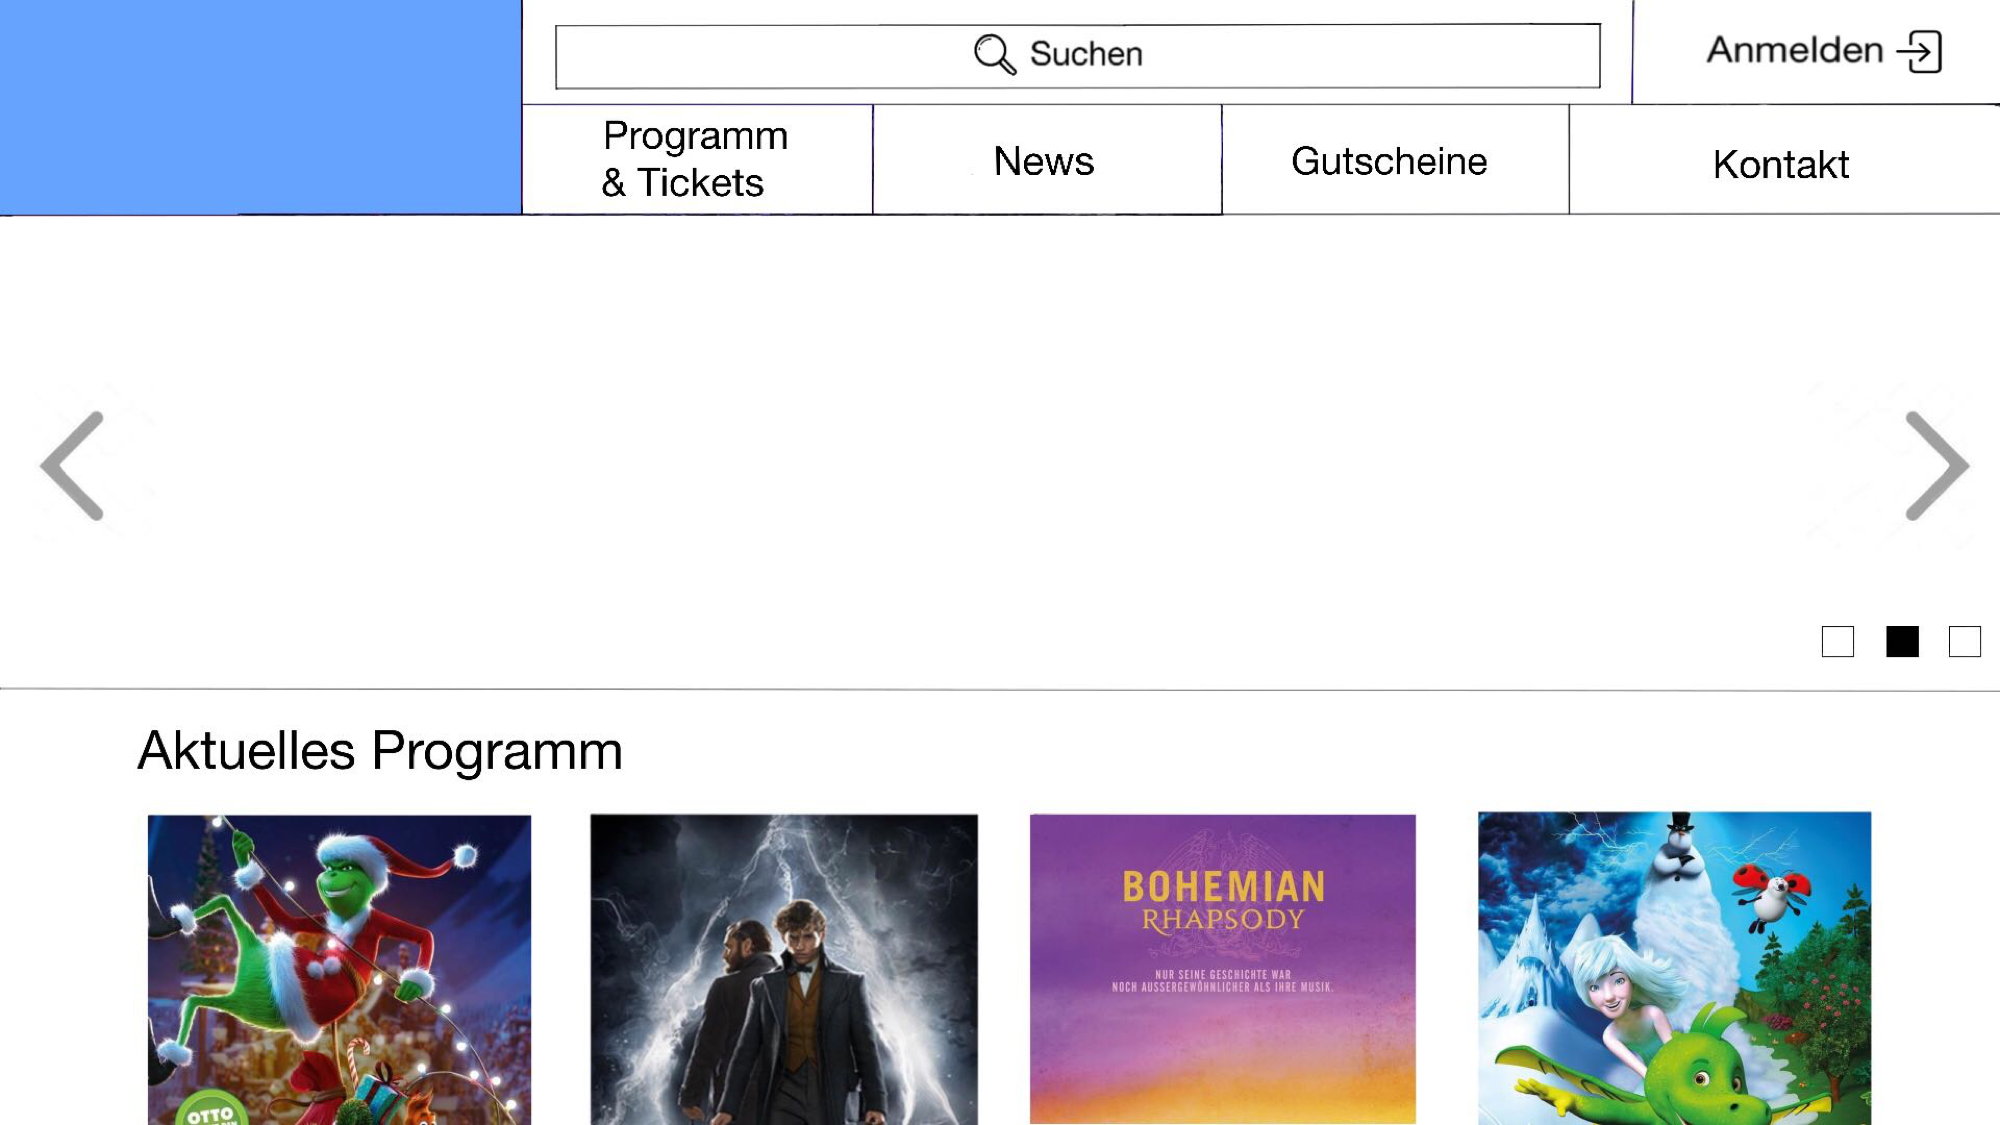
\includegraphics[width=14cm]{img/mockUp1.png}
			\captionsetup{format=hang}
			\caption[Mockup Startseite]{\label{fig:mockUpStartseite} Mockup Startseite }
		\end{figure}
		\begin{figure}[H]
			\centering 
			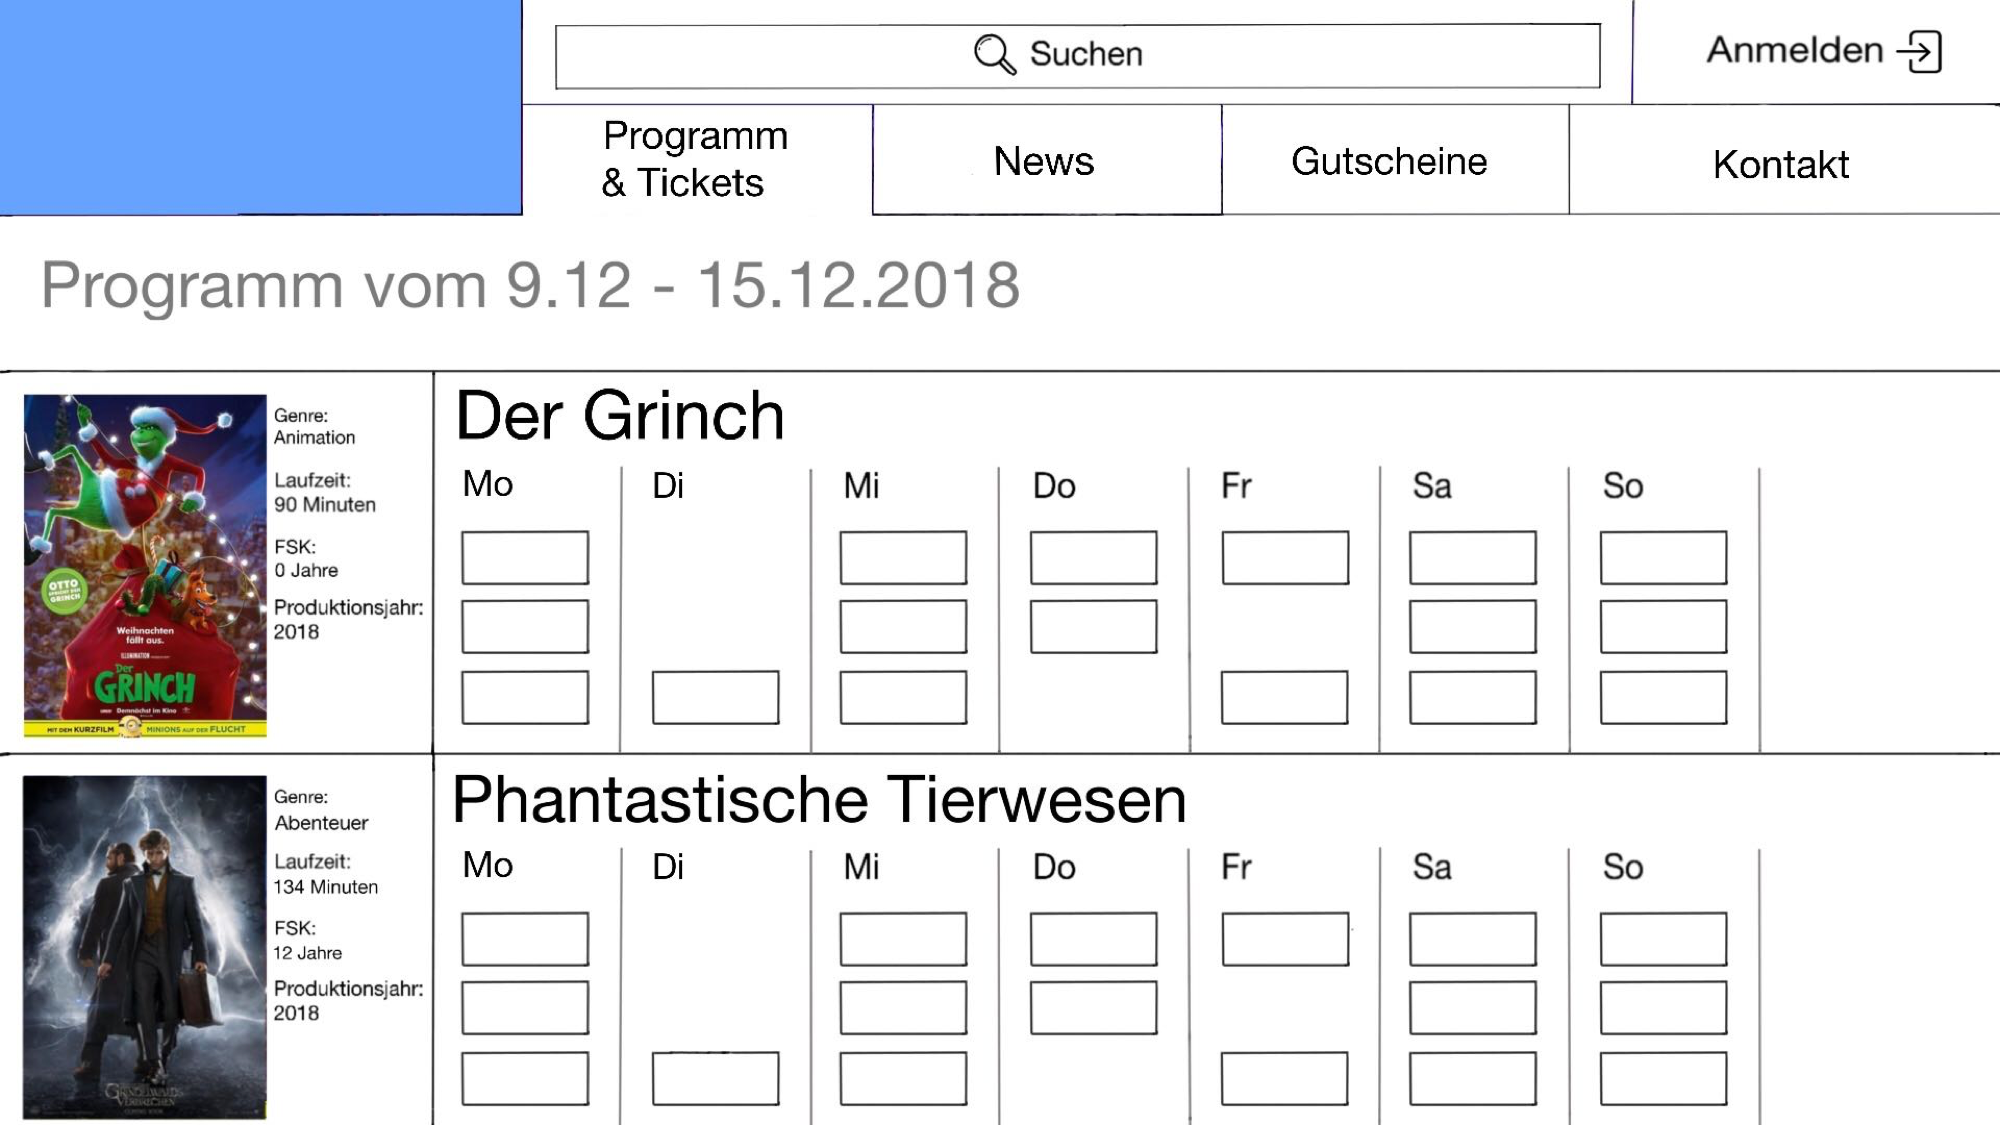
\includegraphics[width=14cm]{img/mockUp2.png}
			\captionsetup{format=hang}
			\caption[Mockup Programm]{\label{fig:mockUpProgramm} Mockup Programm }
		\end{figure}
		\begin{figure}[H]
			\centering 
			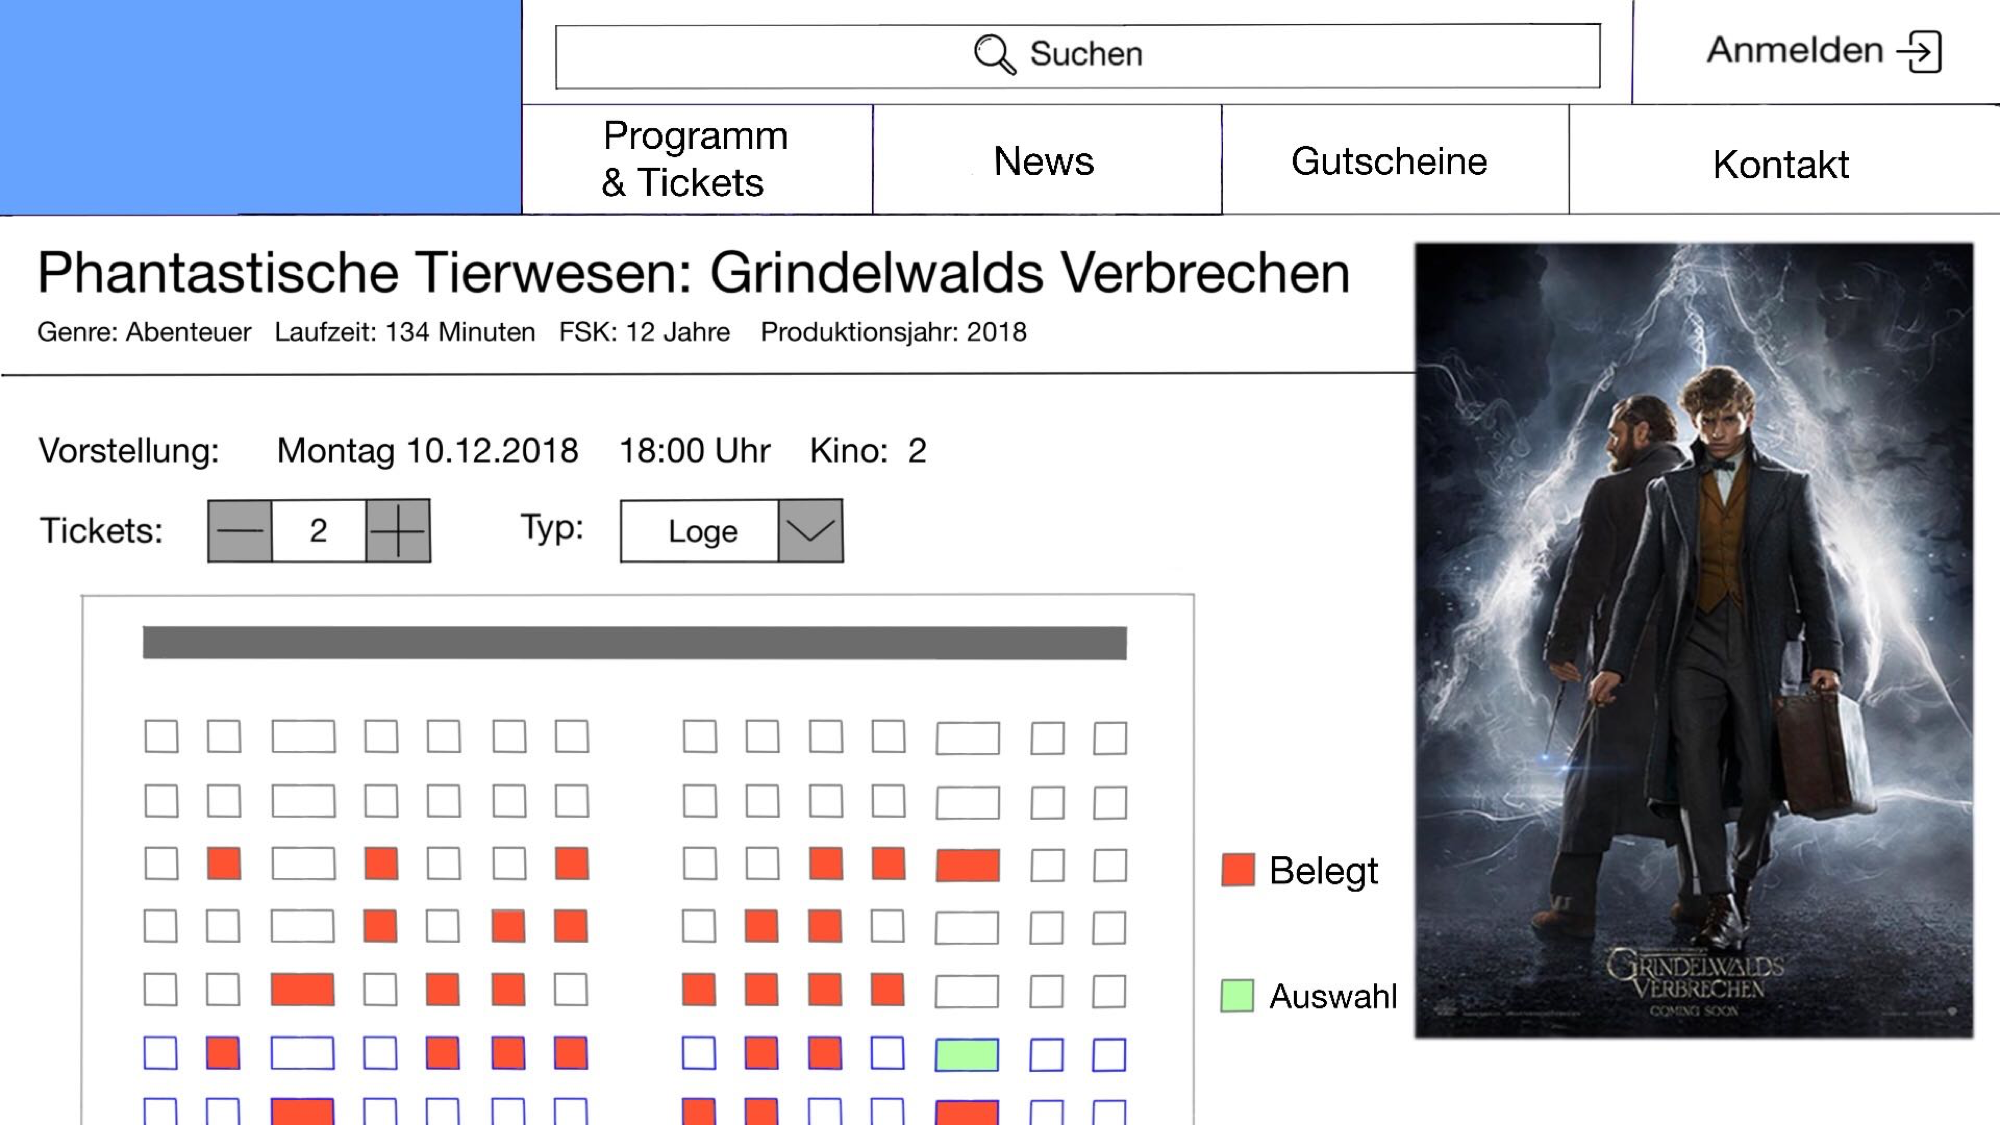
\includegraphics[width=14cm]{img/mockUp3.png}
			\captionsetup{format=hang}
			\caption[Mockup Sitzplan]{\label{fig:mockUpSitzplan} Mockup Sitzplan }
		\end{figure}
	
	\section{Technischer Entwurf} 	
		\subsection{Statische Modelle}
			\begin{figure}[H]
				\centering 
				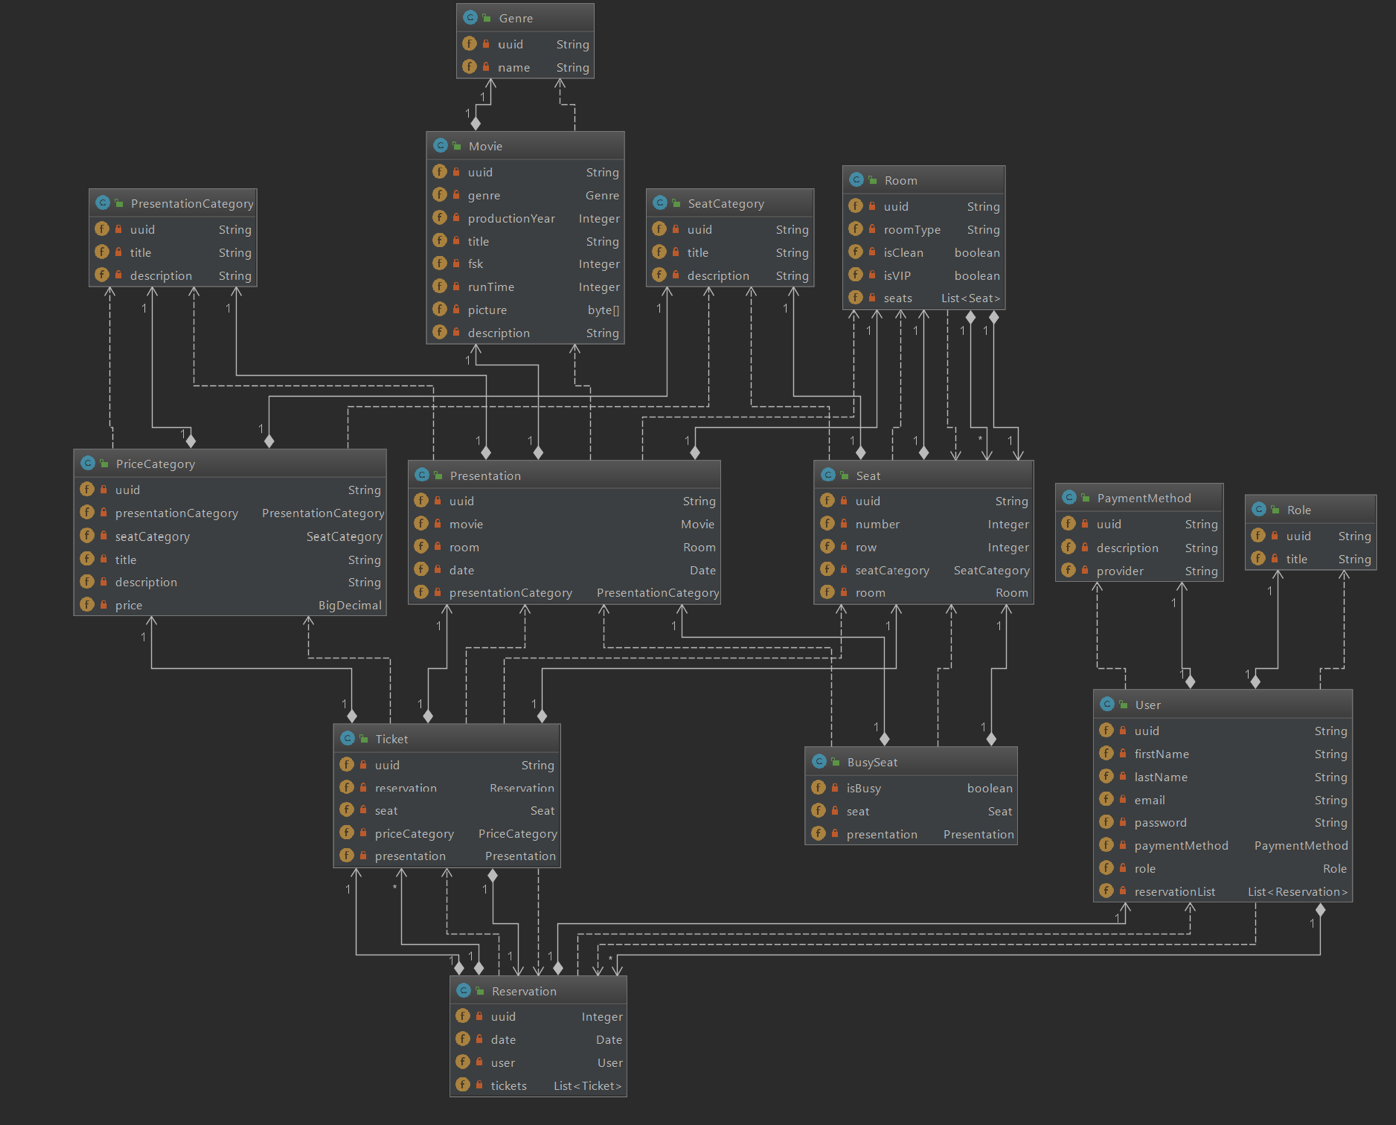
\includegraphics[width=14cm]{img/klassendiagramm.png}
				\captionsetup{format=hang}
				\caption[Klassendiagramm]{\label{fig:klassendiagramm} Klassendiagramm }
			\end{figure}
		
			\begin{figure}[H]
				\centering 
				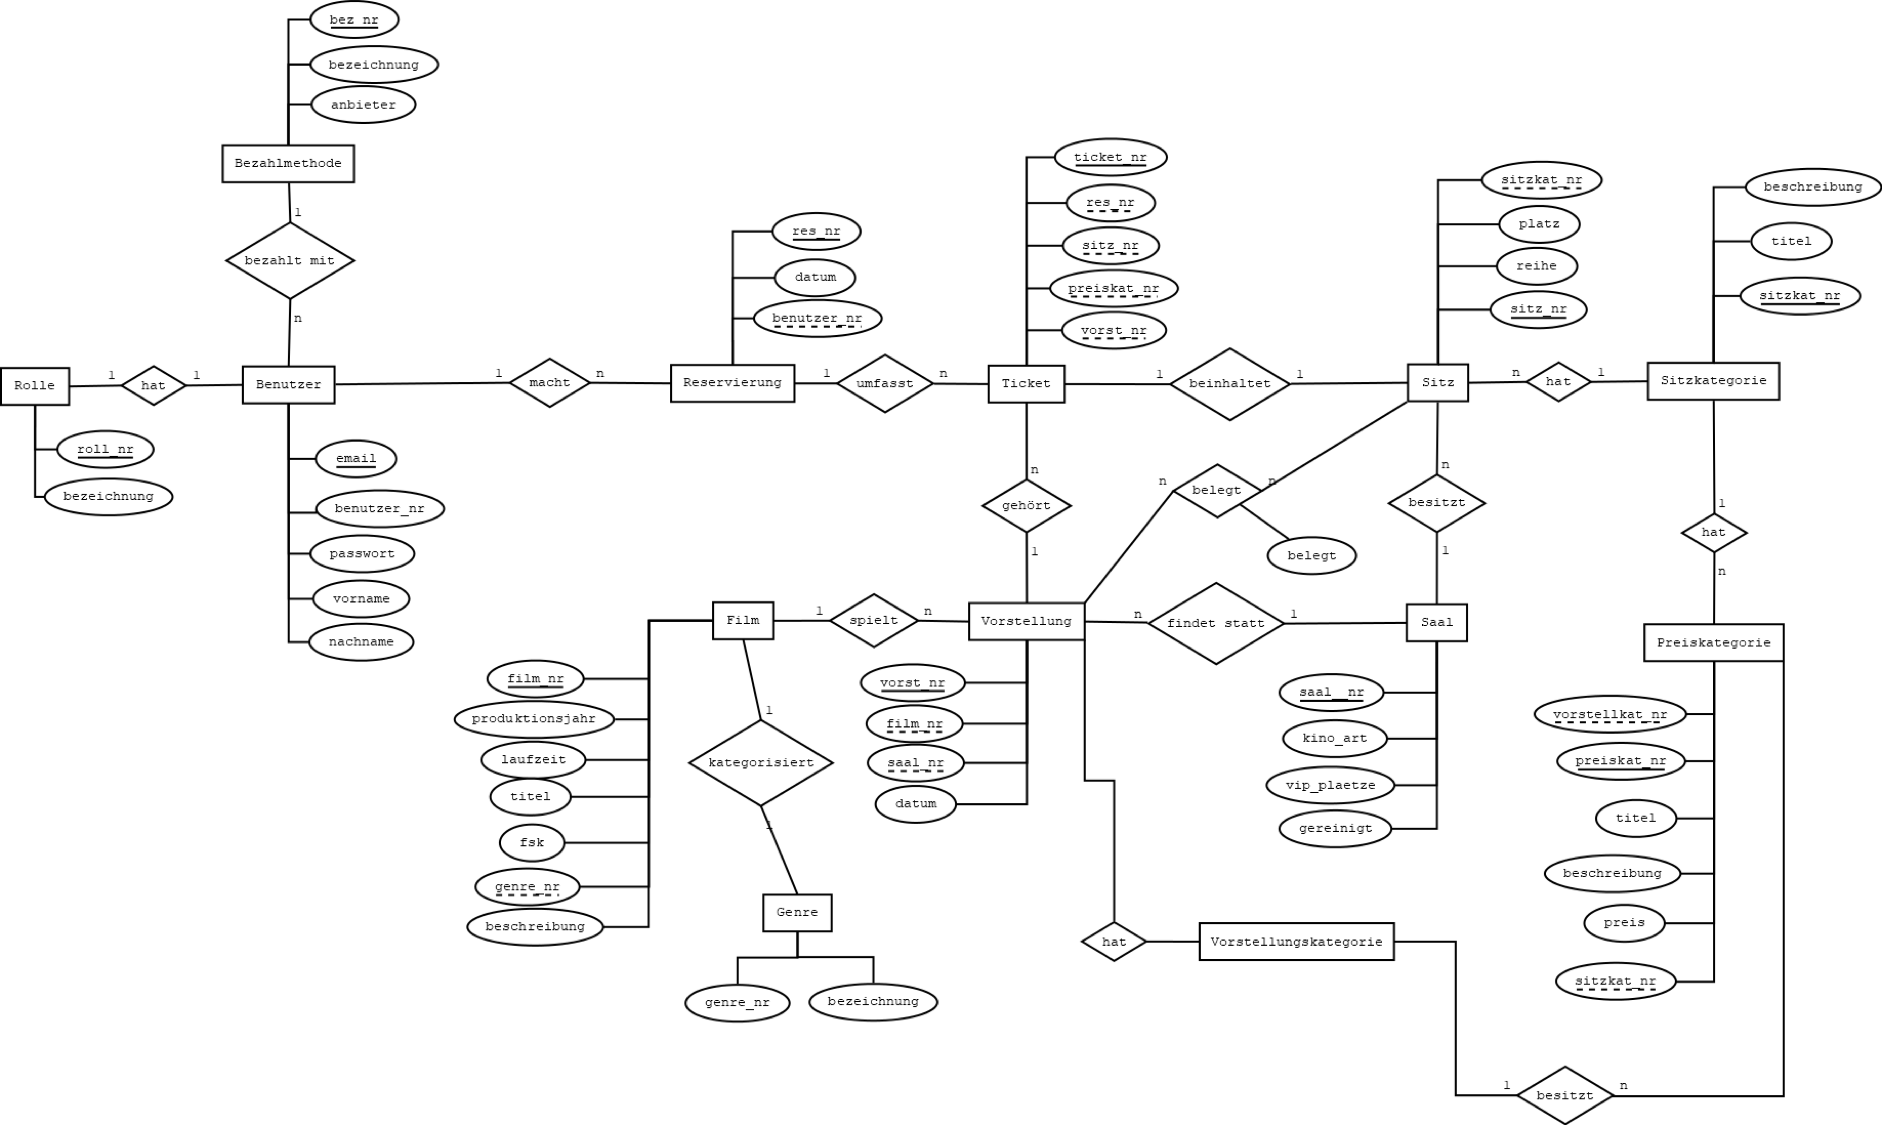
\includegraphics[width=15cm]{img/erModell.png}
				\captionsetup{format=hang}
				\caption[Entity Relationship Datenmodell]{\label{fig:erModell} Entity Relationship Datenmodell}
			\end{figure}
		
		\subsection{Dynamische Modelle}
			\begin{figure}[H]
				\centering 
				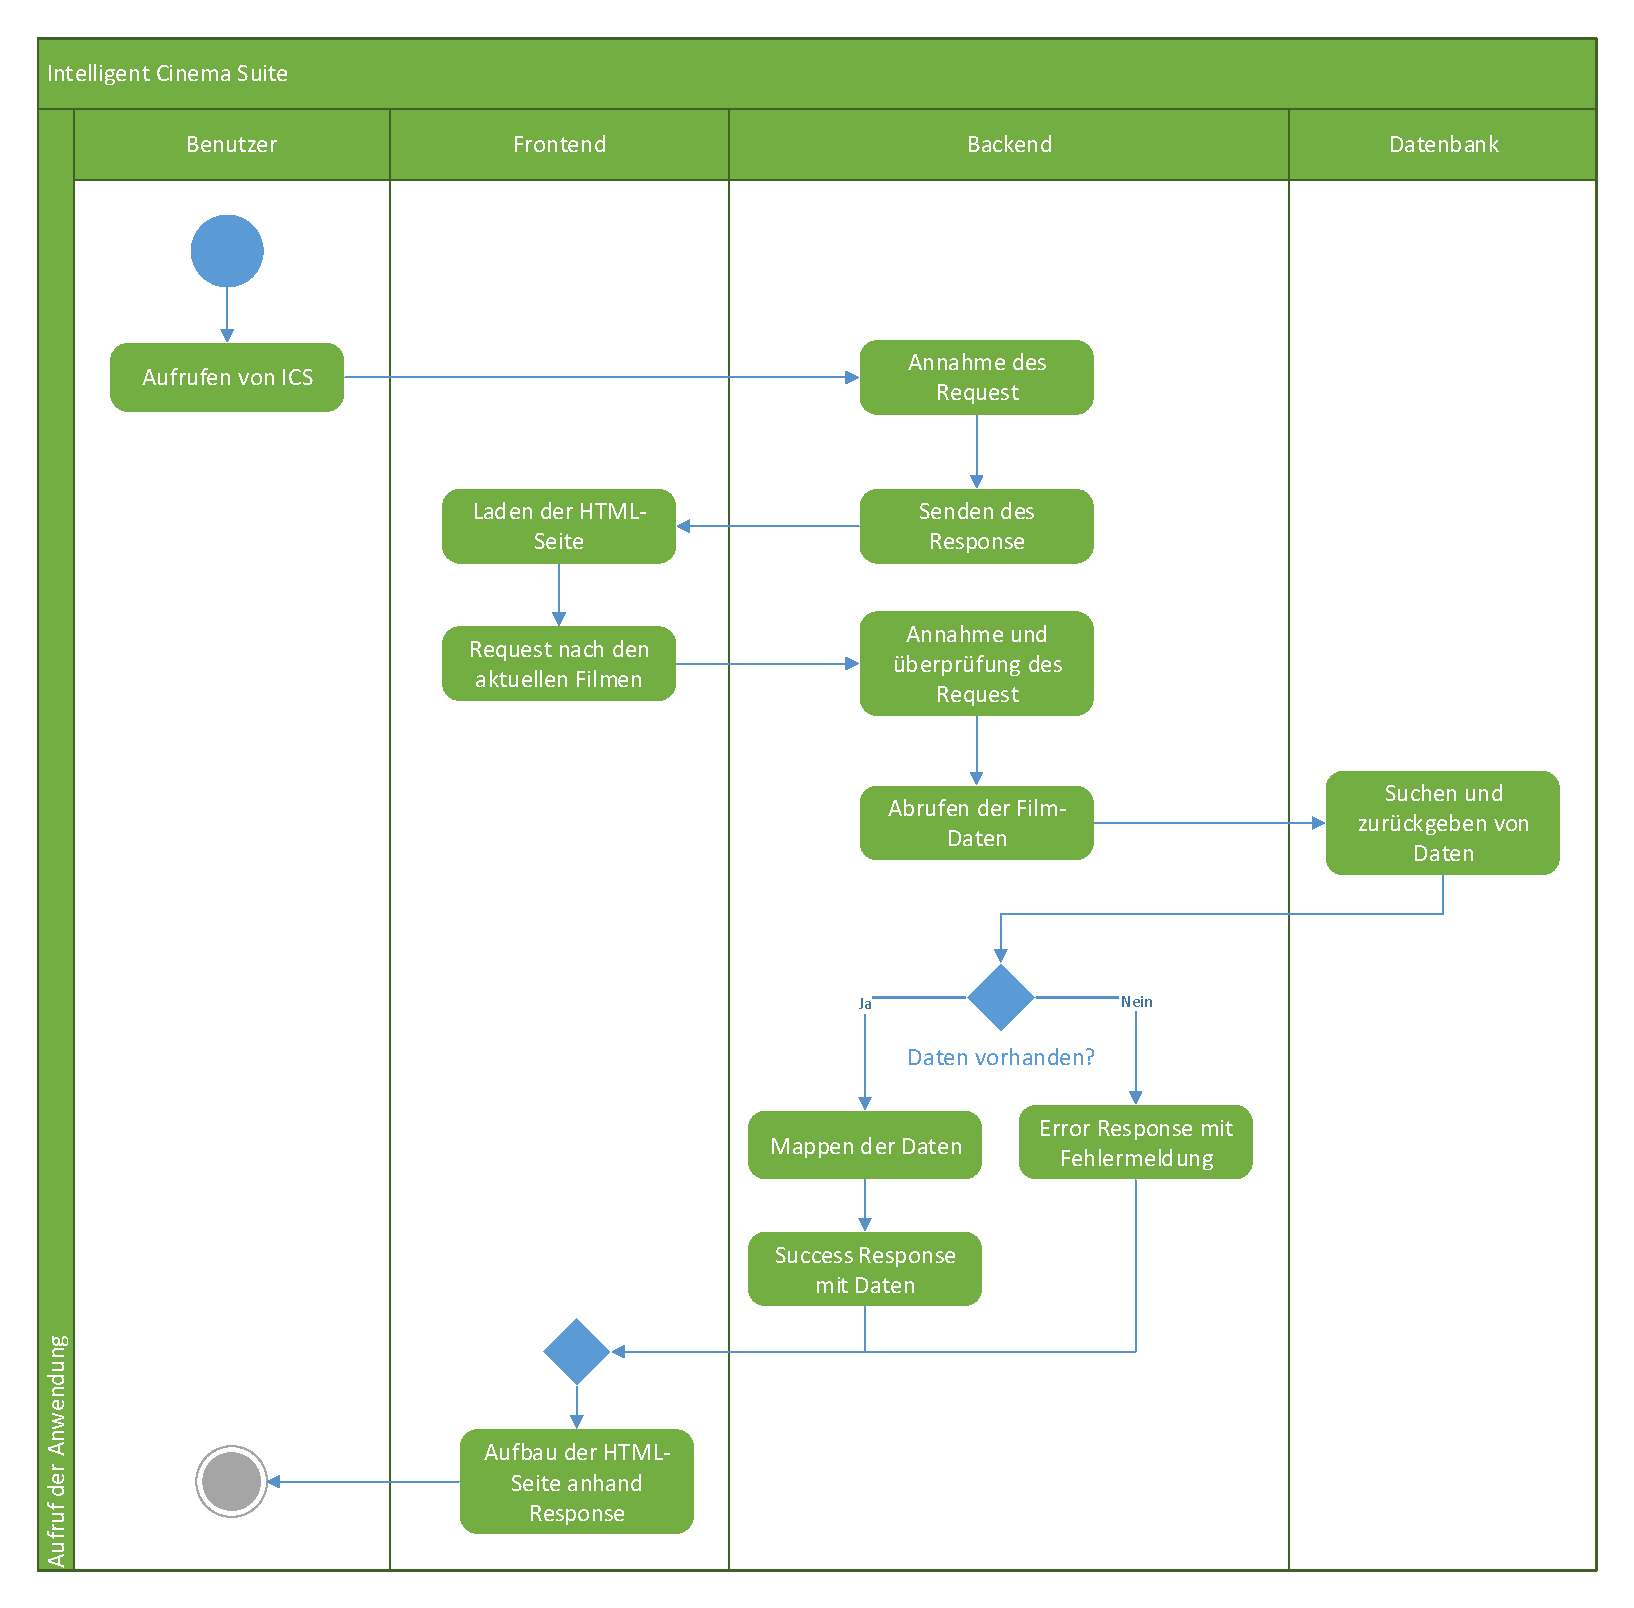
\includegraphics[width=15cm]{img/adSeitenaufruf.pdf}
				\captionsetup{format=hang}
				\caption[Aktivitätsdiagramm Seitenaufruf]{\label{fig:aktivitätSeitenaufruf} Aktivitätsdiagramm Seitenaufruf}
			\end{figure}
		
%			\begin{figure}[H]
%				\centering 
%				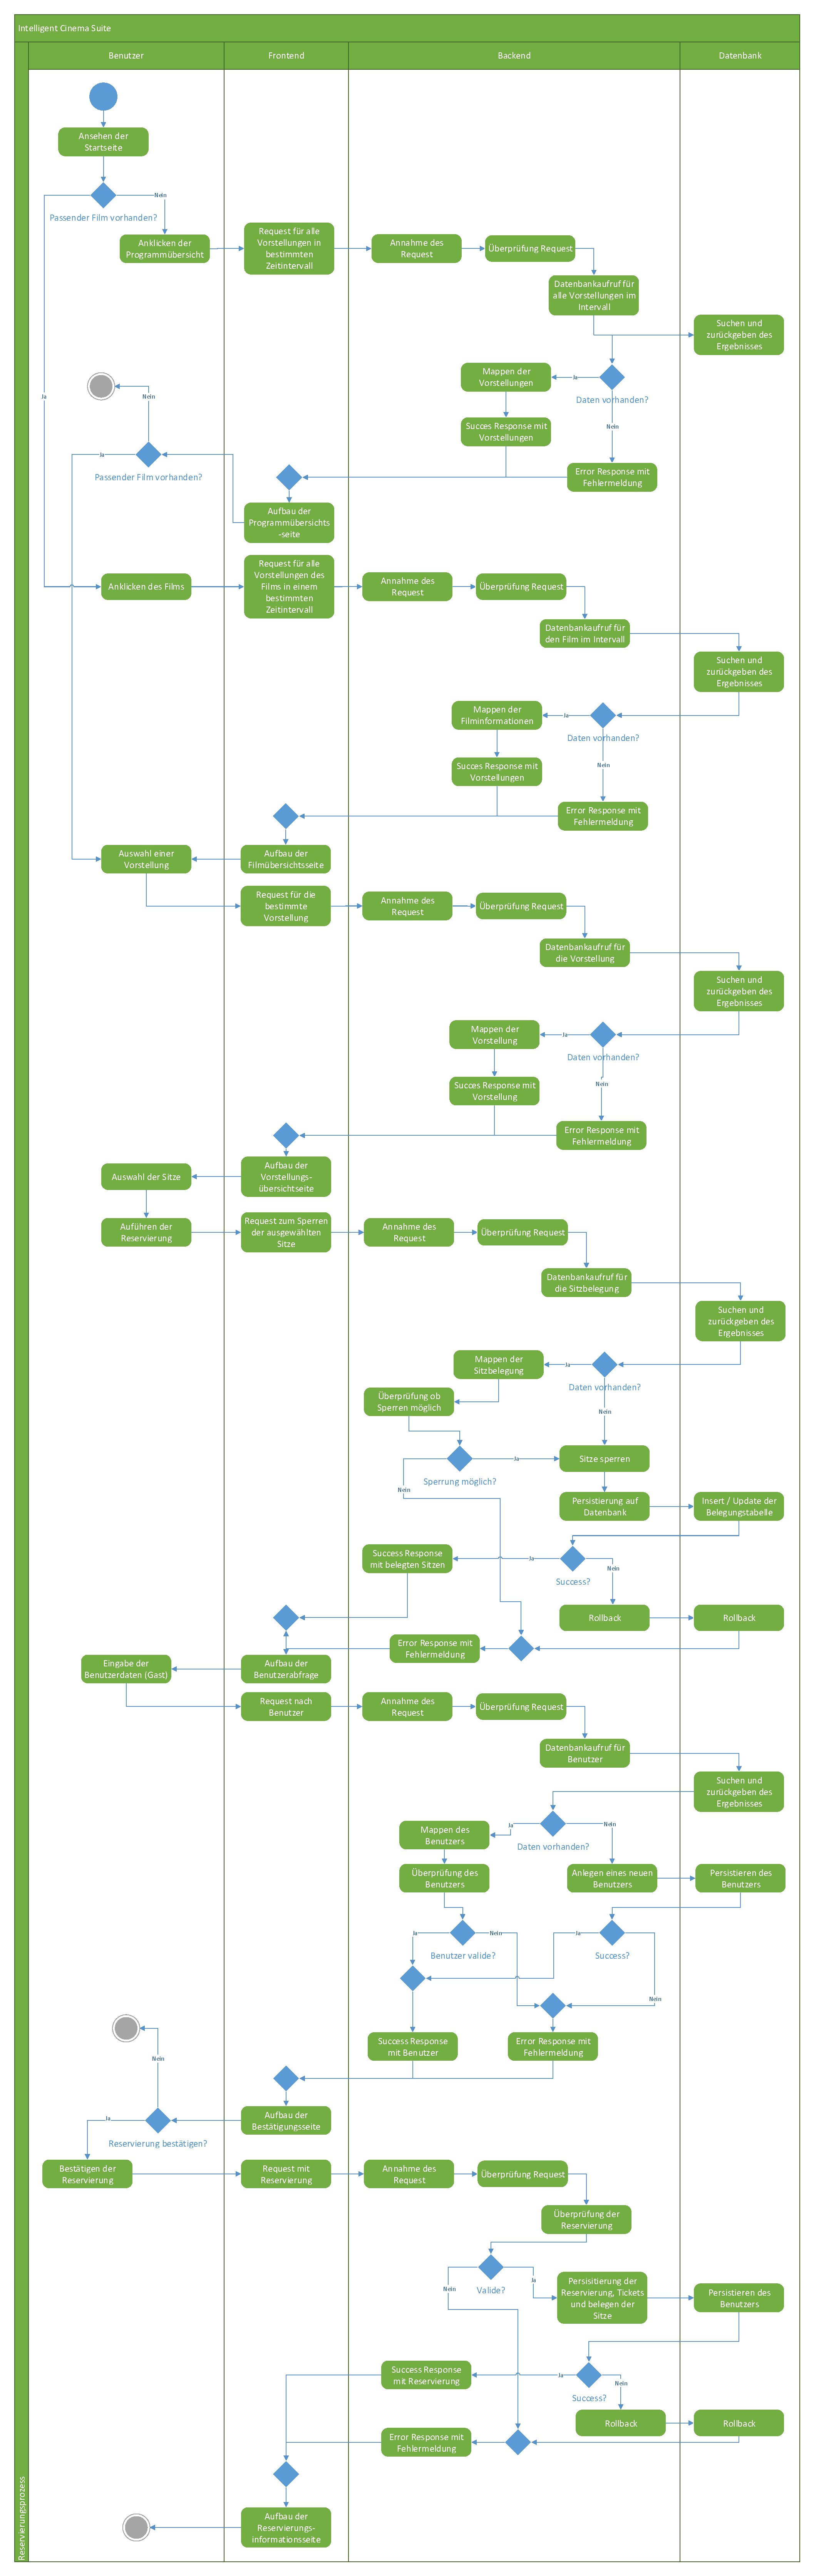
\includegraphics[width=14cm]{img/adReservierung.pdf}
%				\captionsetup{format=hang}
%				\caption[Aktivitätsdiagramm Seitenaufruf]{\label{fig:aktivitätSeitenaufruf} Aktivitätsdiagramm Reservierung}
%			\end{figure}
			
		